\documentclass[tikz,border=10pt]{standalone}
\usetikzlibrary{shapes}
\usetikzlibrary{arrows}
\usetikzlibrary{positioning}
\begin{document} 
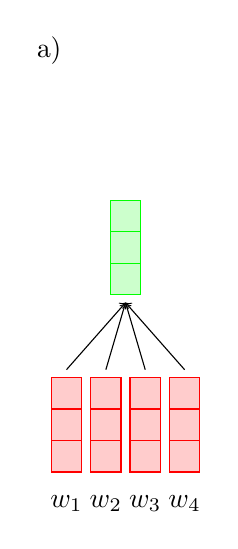
\begin{tikzpicture}[
  hid/.style 2 args={
    rectangle split,
    draw=#2,
    rectangle split parts=#1,
    fill=#2!20,
    outer sep=1mm}]

  \node[hid={3}{green}] (s1) at (1.25, 1.25) {};
  %\node [anchor=west] (label) at (0, 1.75) {a)};
  \node [anchor=west] (label) at (0, 3.75) {a)};
    
  \foreach \i [count=\step from 1] in {1, 2, 3, 4} {
    \node (i\step) at (.5*\step, -2) {$w_\i$};
    \node [hid={3}{red}] (e\step) at (.5*\step, -1) {};    
    \draw [->] (e\step.north) -> (s1.south);
  }
%  \foreach \step in {4,...,6} {
%    \node[hid={3}{red}] (e\step) at (.5*\step, -1) {};    
%    \draw[->] (i\step.north) -> (e\step.south);
%  }
 
 %\node[circle,draw=black] (avgpool) at (1.75, 1) {$+$};
 
%  \foreach \step in {1,...,3} {
%    \node[hid={3}{red}] (e\step) at (.5*\step, -1) {};    
%    \draw[->] (e\step.north) -> (avgpool.south);
%  }
 
 %\draw[->] (avgpool.north)->(s1.south);


\end{tikzpicture}
\end{document}
